% vim: ft=tex iskeyword=@,48-57,_,-,192-255,\: dictionary=bibkeys.lst,labels.lst:
\chapter{Optimization for a Perfect Entangler}
\label{chap:pe}

\section{Introduction}

\section{Models}
\label{sec:pe_models}

We consider the following two-qubit Hamiltonian
\begin{equation}
\begin{split}
  \Op{H}
  &
  =
  \sum_{i}\omega_{i} \Op{\sigma}_{z}^{i}
  +\zeta\Op{\sigma}_{z}^{(1)}\Op{\sigma}_{z}^{(2)}
  + \\ & \quad
  +u(t)\left(
                 \Op{\sigma}_{x}^{(1)}
    +\lambda     \Op{\sigma}_{x}^{(2)}
    +\epsilon_{1}\Op{\sigma}_{x}^{(1)}\Op{\sigma}_{z}^{(2)}
    -\epsilon_{2}\Op{\sigma}_{z}^{(1)}\Op{\sigma}_{x}^{(2)}
  \right)\,,
  \label{eq:pe_fullH}
\end{split}
\end{equation}
with $\Op{\sigma}_{i}^{\left(j\right)}$  the $i$th Pauli operator
acting on the $j$th qubit and $u\left(t\right)$ the control field. We
have shown in paper~I that this Hamiltonian can generate non-trivial
paths in the Weyl chamber. In the following, we discuss how
Eq.~\eqref{eq:pe_fullH} can be used to model qubits based on
superconducting circuits.% as well as nitrogen-vacancy centers.

%% \subsection{NV center}
%% \label{subsec:model:NV}
%% We consider a nitrogen vacancy center with the four states
%% $|00\rangle=|0\rangle_e|0\rangle_n$, $|01\rangle=|0\rangle_e|1\rangle_n$,
%% $|10\rangle=|1\rangle_e|0\rangle_n$, and $|11\rangle=|1\rangle_e|1\rangle_n$,
%% where the electron states $|i\rangle_e$ are determined by $m_s=0,-1$ and the
%% nuclear states by $m_I=-1/2,1/2$. These levels are driven by a radio frequency
%% field $\Omega_{RF}$ and a microwave field $\Omega_{MW}$:
%% %%% please rewrite with the Pauli operator notation
%% \begin{equation}
%%   \label{eq:H_NV}
%%   H_{NV} =
%%   \begin{pmatrix}
%%     0 & 0 & \Omega_{MW}/2 & 0 \\
%%     0 & \omega_{01} & 0 & 0 \\
%%     \Omega_{MW}/2 & 0 & \delta_{MW} & \Omega_{RF}/2\\
%%     0 & 0 & \Omega_{RF}/2 & \delta_{MW}-\delta_{RF}
%%   \end{pmatrix}
%% \end{equation}
%% If we tune the radiation fields on resonance we are left with a microwave driving
%% \begin{equation}
%%  H_{MV}=\frac{\Omega_{MV}}{4}\Op{\sigma}_x^{(1)}\otimes(I+\Op{\sigma}_z)^{(2)}
%% \end{equation}
%% and a radio frequency driving
%% \begin{equation}
%%  H_{RF}=\frac{\Omega_{RF}}{4}(I-\Op{\sigma}_z)^{(1)}\otimes\Op{\sigma}_x^{(2)}\,.
%% \end{equation}

\subsection{Two transmon qubits interacting jointly with a cavity}
\label{subsec:pe_transmon_model}

Two transmons, i.e., anharmonic multi-level systems that interact
jointly with a cavity are described by  a generalized
Jaynes-Cummings Hamiltonian. The  energy of
each transmon qubit transition given by $\omega_1$, $\omega_2$ for the first
(``left'') and second (``right'') transmon respectively.
Higher levels are given as a Duffing oscillator with anharmonicity
$\alpha_1$, $\alpha_2$. Each qubit couples to the cavity with coupling strength
$g_1$ , $g_2$.
In the dispersive limit $|\omega_i -\omega_r| \gg |g{i}|$, $i=1,2$, with
$\omega_r$ the cavity frequency, the cavity can be eliminated and an effective
two-transmon Hamiltonian is obtained. The coupling between each transmon and the
cavity tuns into an effective qubit-qubit coupling
\begin{equation}
J^{\eff}
\approx
    \frac{g_1 g_2}{(\omega_1-\omega_r)}
  + \frac{g_1 g_2}{(\omega_2-\omega_r)}\,.
\end{equation}
In most current setups, $J^{\eff} \ll |\omega_2 - \omega_1|$,
and the two-transmon Hamiltonian can be approximated as \cite{PolettoPRL2012}
\begin{equation}
\begin{split}
  H_{2T}
  &
  \approx
    \sum_{i=1,2} \left(
        \left( \omega_i + \frac{\alpha_i}{2}\right)
        \Op{b}_i^{\dagger} \Op{b}_i
        - \frac{\alpha_i}{2} \left( \Op{b}_i^{\dagger} \Op{b}_i \right)^2
    \right)
  + \\ \quad &
  + J^{\eff} \left( \Op{b}_1^\dagger \Op{b}_2
                  + \Op{b}_1 \Op{b}_2^\dagger
            \right)
  + \\ \quad &
  + \Omega(t) \left( \Op{b}_1 + \Op{b}_1^\dagger
                    + \lambda \Op{b}_2 + \lambda \Op{b}_2^\dagger \right)
\end{split}
\label{eq:PE_H2T}
\end{equation}
where $\Omega(t)$ is the driving field that couples to the cavity and typical
parameters are given in Tab.~{\ref{tab:pe_transmon_parameters}}.

\begin{table}[tb]
  \centering
  \begin{tabular}{llrl} \hline\hline
  left qubit frequency           &  $\omega_1$  & 4.380 &GHz \\
  right qubit frequency          &  $\omega_2$  & 4.614 &GHz \\
  left qubit anharmonicity       &  $\alpha_1$  & -210  &MHz \\
  right qubit anharmonicity      &  $\alpha_1$  & -215  &MHz \\
  effective qubit-qubit coupling &  $J^{\eff}$  & -3.0  &MHz \\
  relative coupling strength     &  $\lambda$   & 1.03  &~\\
  \hline\hline
  \end{tabular}
  \caption{Parameters for the transmon Hamiltonian Eq.~({\ref{eq:PE_H2T}})}.
  \label{tab:pe_transmon_parameters}
\end{table}
%\begin{eqnarray}
  %H_{2Q}&=&\sum_i\frac{\Omega^i}{2}\Op{\sigma}_z^i+\Omega(t)(a+a^+) +\omega_ra^+a
  %\nonumber\\
  %&&+\frac{J^{\eff}}{\omega^2-\omega^1}\Omega(t)
  %\left\{ -g^{1,\eff}\Op{\sigma}^1_z\Op{\sigma}_x^2+g^{2,\eff}\Op{\sigma}_x^1\Op{\sigma}_z^2
  %\right\}\nonumber\\
  %&&+\frac{\left(J^{\eff}\right)^2}{\omega^2-\omega^1}\Op{\sigma}^1_z\Op{\sigma}_z^2
  %+\sum_ig^{i,\eff}\Omega(t)\Op{\sigma}_x^i\,,
%\end{eqnarray}
%where $\Omega^i=\omega^i+2\left(J^{\eff}\right)^2/(\omega^2-\omega^1)$.
An effective two-qubit Hamiltonian is obtained by truncating the higher levels.
This approximation is not necessarily justified, and we  use it only for
interpretation and to analyze controllability, cf.\ paper~I.


\subsection{Charge qubits with Josephson junction coupling}

\label{subsec:pe_charge_model}
\begin{figure}[tb]
  \centering
  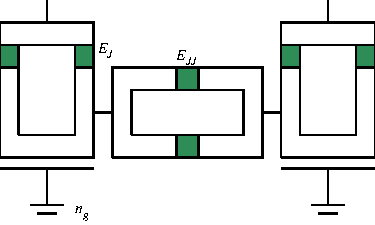
\includegraphics{Josephson-Junction}
  \caption{Setup of the Josephson charge qubits (left and right) coupled by
  a Josepshon junction (middle). The local charge levels are driven by $E_J$.
  The interaction is driven by $E_{JJ}$.
  }
  \label{fig:JCQ-sketch}
\end{figure}

The local Hamiltonian for two Josephson charge qubits reads
\begin{equation}
\begin{split}
  \label{eq:H_charge_loc}
  \Op{H}^{\text{loc}}_C
  &
  =
  \sum_{i=1,2} \sum_{n_i}
  \Bigg[
    E_C \left(n_i -n_g^{(i)}\right)^2 \Ket{n_i}\!\Bra{n_i}
  + \\ & \qquad\quad
    - \frac{E_J^{(i)}}{2}
     \bigg(
      \Ket{n_i}\!\Bra{n_{i} + 1} + \Ket{n_{i}+1}\!\Bra{n_i}
    \bigg)
  \Bigg]\,.
\end{split}
\end{equation}
The interaction is described by
\begin{equation}
  \label{eq:H_charge_int}
  \Op{H}_{JJ}
  = \frac{E_{JJ}}{2}\sum_{n_1,n_2} \left(
    \Ket{n_1}\!\Bra{n_2+1} \Ket{n_1+1}\!\Bra{n_2} + h.c.
    \right)
\end{equation}
Figure~\ref{fig:JCQ-sketch} shows the setup with the two qubits and the
interaction. The local charge levels are driven by $E_J$. The interaction is
driven by $E_{JJ}$. The drift term in the local Hamiltonian depends on the
offset charge $n_g=1$ and the charging energy $E_C$ that works against leakage
to higher levels.


\section{Optimal control using CRAB}
\label{sec:CRAB}

\subsection{Perfect entangler functional in $c$-space}

In the context of the geometric theory for two-qubit gates, reviewed in paper~I,
a functional for finding gates of a given local equivalence class can be
expressed though the difference of the Weyl chamber coordinates of an
obtained gate and the target point,
\begin{equation}
 F_{\lec}=\cos\frac{\Delta c_1}{2}\cos\frac{\Delta c_2}{2}\cos\frac{\Delta
    c_3}{2}\,.
\end{equation}
Building on the local-equivalence class functional, a functional $F_{\PE}$ for
the optimization of an arbitrary perfect entangler can be derived.
In the Weyl chamber, the perfect entanglers form a polyhedron confined by the
three planes
\begin{eqnarray}
 c_1+c_2&=&\pi/2\,,\\
 c_2+c_3&=&\pi/2\,\quad\text{and}\\
 c_1-c_2&=&\pi/2\,.
\end{eqnarray}
These planes divide the Weyl chamber into the polyhedron of perfect entanglers
and three corners of non-perfect entanglers. Within the perfect-entangler
polyhedron, the fidelity of a unitary gate $U$ within is defined $F_{\PE}(U)
\equiv 1$. Outside of polyhedron, the value of $F_{\PE}$ depending on the region
of the Weyl chamber the gate is in,
\begin{eqnarray}
 F_{\PE}(U)=\begin{cases}
\cos^2\frac{c_{U,1}+c_{U,2}-\frac{\pi}{2}}{4}\,,\qquad c_1+c_2\leq\frac{\pi}{2}\\
\cos^2\frac{c_{U,2}+c_{U,3}-\frac{\pi}{2}}{4}\,,\qquad c_2+c_3\geq\frac{\pi}{2}\\
\cos^2\frac{c_{U,1}-c_{U,2}-\frac{\pi}{2}}{4}\,,\qquad c_1-c_2\geq\frac{\pi}{2}\\
1\qquad\text{otherwise (inside polyhedron).}
          \end{cases}
\end{eqnarray}
Both $F_{\lec}$ and $F_{\PE}$ take values in $[0,1]$ and can thus be interpreted
as fidelities.

Generally, the logical two-qubit subspace is embedded in a larger Hilbert space,
such that while the dynamics in the total Hilbert space are unitary, the
dynamics in the subspace may not be. In this case,
a closest unitary $U$ can be derived from the non-unitary (projected) gate
$\tilde{U}$: If $\tilde{U}$ has the singular value decomposition
$\tilde{U} = V \Sigma W^{\dagger}$, then the unitary that fulfills
$U = \arg \min_{u} \Vert u-\tilde{U} \Vert$ is given by $U = V W^\dagger$.
The local-equivalence-class and perfect-entangler fidelities then becomes
\begin{eqnarray}
F_{\lec}((\tilde U) = F_{\lec}(U) -||\tilde U -U||\,,\label{eq:FUtilde-lec}\\
F_{\PE}(\tilde U) = F_{\PE}(U) -||\tilde U -U||\,.\label{eq:FUtilde-pE}
\end{eqnarray}
This fidelity can be directly used as optimization functional so that the
optimization target is to find $c_i$ in such a way that
Eqs.~(\ref{eq:FUtilde-lec},~\ref{eq:FUtilde-pE}) are maximized.


\subsection{CRAB algorithm}

The chopped random basis (CRAB) algorithm is an optimal control tool that
allows to optimize quantum operations in situations where it is either not
possible or impractical to calculate gradients of the optimization functional.
Originally it was developed in the context of quantum
many body systems \cite{DoriaPRL11,CanevaPRA11} where the gradient evaluation
is too time-consuming.
In the context of this paper, it is mathematically unfeasible to calculate
gradients of $F_{\lec}$ and $F_{\PE}$ as given in
Eqs.~(\ref{eq:FUtilde-lec},~\ref{eq:FUtilde-pE}) with respect to the states
(as needed for the Krotov update formula in Sec~\ref{sec:Krotov} below),  since
the functionals depends on the states in a highly non-trivial way.

The central idea of CRAB is the expansion of the control function into
a truncated basis using random basis functions
\begin{equation}
 u(t)=\sum_{i=1}^n c_i f_i(t)\,
\end{equation}
where the set of $f_i$ form the truncated basis.
We choose $f_i=\sin (\omega_i t)$
with random $\omega_i\in [\frac{2\pi i}{T}-0.5,\frac{2\pi i}{T}+0.5]$.
Then, the coefficients $c_i$ are optimization by a direct search
algorithm, Nelder-Mead downhill simplex in our case.


\section{Optimal control using Krotov's method}
\label{sec:Krotov}

\subsection{Perfect entangler functional in $g$-space}
\label{subsec:imp_Krotov}

For optimal control approaches such as Krotov's method~\cite{ReichJCP12},
the gradient of the optimization functional needs to be evaluated. Specifically,
for Krotov the derivative with respect to the states is required.
The functionals of Eqs.~(\ref{eq:FUtilde-lec},~\ref{eq:FUtilde-pE}),
do not straightforwardly allow to evaluate this derivative.
As shown in paper~I, we must therefore use an equivalent
functional, based not on the Weyl space coordinates $c_1$, $c_2$, $c_3$, but on
the local invariants $g_1$, $g_2$, $g_3$.

For the local invariants, an appropriate functional is
\begin{equation}
  \label{eq:J_T_li_g}
  J_{\LI}(U) = (\Delta g_1)^2 + (\Delta g_2)^2 + (\Delta g_3)^2\,,
\end{equation}
where $\Delta g_i$ is the Euclidean distance between local invariant $g_i$ of
the obtained unitary $U$ and the optimal gate $O$.
For the perfect entanglers, the functional becomes
\begin{equation}
  \label{eq:J_T_pe_g}
  \mathcal{D}(U)
      =  g_3 \sqrt{g_1^{2} + g_2^{2}} - g_1
\end{equation}
Both of these functionals take the value zero if the goal is reached, and are
thus distance measures, as opposed to the fidelities in
Eqs.~(\ref{eq:FUtilde-lec},~\ref{eq:FUtilde-pE}). Specifically, they are not in
the range $[0,1]$.

Again, we must take into account non-unitarity due to projection onto the logical
subspace. Just as for the functionals, the expression $||\tilde U -U||$
used in Sec~\ref{sec:CRAB} cannot easily be differentiated. As an alternative,
we minimize the loss of population $\Tr\left[ \tilde U^\dagger \tilde U \right]/4$
from the logical subspace.
\begin{eqnarray}
J_{\LI}(\tilde U)
= w J_{\LI}(U) + (w-1)\left(1 - \frac{1}{4} \Tr\left[ \tilde U^\dagger \tilde U \right]\right)
\label{eq:J_LI_tilde}\\
\mathcal{D}(\tilde U)
= w \mathcal{D}(U) + (w-1) \left(1 - \frac{1}{4} \Tr\left[ \tilde U^\dagger \tilde U \right]\right)
\label{eq:J_pe_tilde}
\end{eqnarray}
In order to weight the relative importance of the Weyl-chamber optimization and
the unitarity, the factor $w \in [0,1]$ is used. This factor can be adaptively
changed during the optimization in order to improve convergence.

\subsection{Krotov's Method}
\label{subsec:KrotovAlgo}

In order to derive an update equation, the total functional $J$ for Krotov's
method must include a control-dependent running cost. The total functional takes
the form
\begin{equation}
  \label{eq:J_krotov}
  J =
  J_T\left[\{\vphi_k(T)\}\right]
  + \int_0^T   \frac{\lambda_a}{S(t)}
    \left[ u(t) - u_\mathrm{ref}(t)\right]^2  \;dt \,,
\end{equation}
where $J_T$ is a final-time functional, e.g.\
Eqs.~(\ref{eq:J_LI_tilde},~\ref{eq:J_pe_tilde}) and the second term is
a constraint on the optimized control field $u(t)$ in each iteration of the
optimization algorithm. Generally, the reference field $u_{\mathrm{ref}}(t)$ is
taken to be the field from the previous iteration.

A comprehensive description of Krotov's method for general quantum control
problems is found in Ref.~\cite{ReichJCP12}. Here, we state the control
equations for a final-time functional $J_T$ that depends higher than
quadratically on the states, linear coupling to the control and linear equations
of motion. In this case, the  update equation for the control at the $i+1$st
iterative step,
$u^{(i+1)}(t)$,  is given by
\begin{equation}
\label{eq:newu}
  u^{(i+1)}(t)
  =
  u_\mathrm{ref}(t) +
  \frac{S(t)}{\lambda}
  \mathfrak{Im} \bigg\{\sum_{k=1}^4 \left\langle \chi_k^{(i)}(t)\Bigg|
      \frac{\partial \Op{H}}{\partial u}
      \bigg|_{u^{(i+1)}}
      \Bigg| \vphi_k^{(i+1)}(t)\right\rangle
   +\frac{1}{2}  \sigma(t)\sum_{k=1}^4
    \left\langle \Delta\vphi_k(t) \Bigg|
      \frac{\partial\Op{H}}{\partial u}\bigg|_{u^{(i+1)},}
      \Bigg|\vphi_k^{(i+1)}(t)\right\rangle \bigg\}
\end{equation}
with
$\Ket{\Delta\vphi_k(t)}=\Ket{\vphi_k^{(i+1)}(t)}-\Ket{\vphi_k^{(i)}(t)}$
representing the  change in state $\Ket{\vphi_k(t)}$.
In Eq.~\eqref{eq:newu}, $S(t)$ is a shape function to smoothly
switch the control on and off, and $\lambda$ is a parameter that
determines the step size of the change in the control. The scalar
function $\sigma(t)$ is constructed to ensure monotonic
convergence. For final-time functionals that depend higher than
quadratically on the states $|\vphi_k(T)\rangle$, linear equations of
motion and linear coupling to the control, it reads~\cite{ReichJCP12}
\begin{equation}
  \label{eq:sigma}
  \sigma(t) = -\bar{A}
\end{equation}
with $\bar{A}=\max\left(\varepsilon_A,2A+\varepsilon_A\right)$, where
$\varepsilon_A$ is a small non-negative number that can be used to
enforce strict inequality in the second order optimality condition.
The parameter $A$ depends on the final-time functional. In principle, it is
possible to determine a supremum for $A$ that guarantees convergence. In
practice, one should determine the optimal value for $A$ in each iteration
numerically as \cite{ReichJCP12}
\begin{eqnarray}
  \label{eq:A_n}
  A^{(i+1)}  & =&
  \frac{\sum_{k=1}^{4}\left[
      \Braket{\chi_k\left(T\right)|\Delta\vphi_k\left(T\right)}
      +\Braket{\Delta\vphi_k\left(T\right)|\chi_k\left(T\right)}\right]
    +J_T\left(\{\varphi_k^{(i+1)}(T)\}\right)
    -J_T\left(\{\varphi_k^{(i)}(T)\}\right)}
  {\sum_{k=1}^{4}\left[
      \Braket{\Delta\vphi_k\left(T\right)|\Delta\vphi_k\left(T\right)}\right]}
  \,.
\end{eqnarray}

Evaluation of the update equation for the control,
Eq.~\eqref{eq:newu}, implies forward
propagation of the logical basis states and backward propagation of
the adjoint states. The forward propagation of the logical basis uses
the new control, as indicated by the superscript $(i+1)$,
\begin{subequations}\label{eq:forward_prop}
\begin{eqnarray}
  \frac{d}{dt}|\vphi^{(i+1)}_k(t)\rangle &=&
  -\frac{i}{\hbar}\Op{H}[u^{(i+1)}]
  |\vphi^{(i+1)}_k(t)\rangle \\
  |\vphi^{(i+1)}_k(0)\rangle &=& |k\rangle \,,\quad k=1,\ldots, 4   \,.
\end{eqnarray}
\end{subequations}
The adjoint states are propagated backward in time under the old
control, $u^{(i)}$,
\begin{subequations}\label{eq:pe_backward_prop}
  \begin{eqnarray}\label{eq:chidot}
  \frac{d}{dt}|\chi^{(i)}_k(t)\rangle &=&
  -\frac{i}{\hbar}\Op{H}^{\dagger}[u^{(i)}]
  |\chi^{(i)}_k\rangle  \\
  |\chi^{(i)}_k(T)\rangle &=& -\nabla_{\Bra{\vphi_k}}
  J_T\big|_{|\vphi^{(i)}_k(T)\rangle}
  \, \label{eq:chiT}
  \end{eqnarray}
\end{subequations}
for the $k = 1 \dots 4$ states that constitute the logical two-qubit basis.
Note that is is Eq.~(\ref{eq:chiT}) that necessitates a functional that is
differentiable with respect to the states.
The initial condition for the adjoint states is given in terms of the
final-time functional, $J_T$. We use either one of of the functionals in
of Eqs.~(\ref{eq:J_LI_tilde},~\ref{eq:J_pe_tilde}).


\section{Applications}
\label{sec:appl}

%% \subsection{Optimization of NV centers}
%% \label{subsec:NV}
%% \begin{figure}[tb]
%%   \centering
%%   \includegraphics{NV-2pulses-polyhedron}
%%   \caption{Reachable gates in the Weyl chamber for an NV center with 2 control
%%   pulses. Each blue dot corresponds to one reached gate at final time. A two
%%   dimensional subspace of the Weyl chamber can be accessed.
%%   }
%%   \label{fig:NV-2pulses}
%% \end{figure}
%%
%% \begin{figure}[tb]
%%   \centering
%%   \includegraphics{NV-3pulses-polyhedron}
%%   \caption{Reachable gates in the Weyl chamber for an NV center with 3 control
%%   pulses. Each blue dot corresponds to one reached gate at final time. All
%%   points in the Weyl chamber can be reached.
%%   }
%%   \label{fig:NV-3pulses}
%% \end{figure}
%% The part of the Weyl chamber we can generate is given by the operators in the
%% Hamiltonian and their commutators. The relevant operators are (on resonance,
%% that is just off-diagonal terms)
%% $$A_1=\Op{\sigma}_x^{(1)}\otimes (I+\Op{\sigma}_z)^{(2)}$$
%% from the microwave pulse and
%% $$A_2=(I-\Op{\sigma}_z)^{(1)}\otimes \Op{\sigma}_x^{(2)}$$
%% from the radio frequency pulse.
%% The commutator is $$A_3=[A_1,A_2]=-\Op{\sigma}_x^{(1)}\Op{\sigma}_y^{(2)} -\Op{\sigma}_y^{(1)}\Op{\sigma}_x^{(2)}\,.$$
%% From here we have $[A_1,A_3]=-A_2$ and $[A_2,A_3]=A_1$. Therefore we have the operators
%% $$\Op{\sigma}_x^{(1)}I^{(2)}+\Op{\sigma}_x^{(1)}\Op{\sigma}_z^{(2)},\space~I^{(1)}\Op{\sigma}_x^{(2)}-\Op{\sigma}_z^{(1)}\Op{\sigma}_x^{(2)}\space~\text{and}\space~ \Op{\sigma}_x^{(1)}\Op{\sigma}_y^{(2)} +\Op{\sigma}_y^{(1)}\Op{\sigma}_x^{(2)}\,.$$
%% Although we have found three different operators, they can't cover the whole
%% Weyl chamber. Figure~\ref{fig:NV-2pulses} shows results for this Hamiltonian and
%% optimization toward the polyhedron of perfect entanglers by CRAB. Also reached
%% gates with low fidelity (e.g.\ from the first few iterations of the simplex) are
%% plotted to see which points in the Weyl chamber are accessible. Clearly, we are
%% limited to two dimensions. At first glance this seems surprising, but indeed
%% $A_1,A_2,A_3$ are linearly dependent up to local transformations and thus span
%% only two dimensions of the Weyl chamber.
%%
%% If we add also a detuning term ($\mathrm{diag}(0,0,0,1)\,\times\,$control),
%% however, we can cover the whole Weyl chamber (Fig.~\ref{fig:NV-3pulses}).
%%
%% The figures show that as long as the system gives enough freedom the algorithm
%% can drive us to whatever point in the Weyl chamber or in the polyhedron of
%% perfect entanglers that yields a good fidelity and thus the results prove that
%% the algorithm works.


\subsection{Optimization of Josephson Charge Qubits}
\label{subsec:JCQ}

As a first application, we optimize the system described in
Sec.~\ref{subsec:pe_charge_model} using the CRAB algorithm.
%
\begin{figure}[tb]
  \centering
  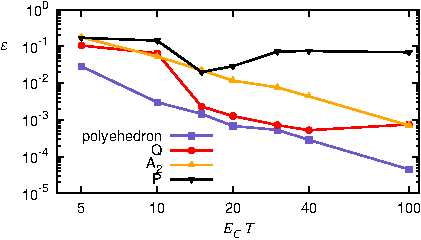
\includegraphics{JCQ-1pulse}
  \caption{Success of optimization of two Josephson charge qubits coupled by
  a Josephson junction. Control with one pulse $E_J(t)=E_{JJ}(t)$. The error
  $\errPE$ for the optimization toward the polyhedron of perfect
  entanglers (blue) is compared to the error $\errLec$ from optimization toward
  specific local equivalence classes, namely $Q$ (red, circles), $A_2$ (yellow,
  triangles pointing upwards), and $P$ (black, triangles pointing downwards).}
  \label{fig:JCQ-fidelity-1pulse}
\end{figure}
%
\begin{figure}[tb]
  \centering
  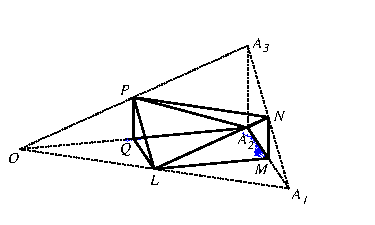
\includegraphics{JCQ-1pulse-polyhedron}
  \caption{Optimized gates in the Weyl chamber. Control with one pulse
  $E_J(t)=E_{JJ}(t)$. Each blue dot corresponds to one reached gate at final
  time. Only a 1D subset of the Weyl chamber can be reached.
  }
  \label{fig:JCQ-1pulse_weyl_paths}
\end{figure}
%
First, we consider constant $E_{JJ}(t)=E_J(t)$, i.e.\ use only one control pulse.
Fig.~\ref{fig:JCQ-fidelity-1pulse} shows the optimization success of the
perfect-entanglers functional for different gate durations in terms of
Eq.~(\ref{eq:FUtilde-lec}) for optimization towards a given local equivalence
class, and Eq.~(\ref{eq:FUtilde-pE}) for optimization towards the polyhedron of
perfect entanglers.
The figure shows the resulting fidelity error
$\errPE(\tilde U)=1-F_{\PE}(\tilde{U})$ for optimization towards the polyhedron of
perfect entanglers (blue, squares) and compares it to the fidelity error
$\errLec(\tilde U)=1-F_{\lec}(\tilde{U})$ for optimization towards a specific perfect
entangler equivalence class. The operation errors are plotted as a function of
$E_C T$, that is the relative strength of the charge energy that splits the
local charge levels or alternatively the operation time. For higher values of
this energy splitting (faster gates) the operation
can clearly be performed with a higher fidelity since it is much easier to
distinguish between two levels and because the charge energy works against
leakage to higher levels.
Considering the generating Hamiltonian this is also to
say that the drift Hamiltonian is important to achieve the desired entangling
gates.
For gates on the time scale of a few nanoseconds $E_C$ has to be of the order of
$1\,$GHz. We put no constraints on the strength control pulses $E_{JJ}(t)$ and
$E_J(t)$ and obtain a pulse strength of the optimized pulses of a few hundred
MHz.

We examined three corners of the polyhedron, namely $Q$ (red, circles), $A_2$
(yellow, triangles pointing upwards), and $P$ (black, triangles pointing
downwards). Clearly the best results are the ones for perfect entangler
optimization. While $Q$ and $A_2$ are reached with pretty high fidelity, $P$ can
not be reached at all. This is also supported by
Fig.~\ref{fig:JCQ-1pulse_weyl_paths} that shows the position in the Weyl chamber
of the gates reached during optimization. Each blue dot corresponds to one reached
gate at final time. Only one dimension (and its vicinity) of the Weyl chamber
can be explored by this setup.

\begin{figure}[tb]
  \centering
  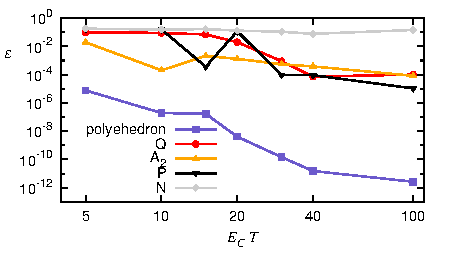
\includegraphics{JCQ-2pulses}
  \caption{Success of optimization of 2 Josephson charge qubits coupled by
  a Josephson junction. Control with 2 pulses $E_J(t)$ and $E_{JJ}(t)$. The gate
  error $\errPE$ for the optimization towards the polyhedron of perfect
  entanglers (blue) is compared to the errors $\errLec$from optimization towards
  specific local equivalence classes, namely $Q$ (red, circles), $A_2$ (yellow,
  triangles pointing upwards), $P$ (black, triangles pointing downwards), and
  $N$ (gray, diamonds).}
  \label{fig:JCQ-fidelity-2pulses}
\end{figure}
%
\begin{figure}[tb]
  \centering
  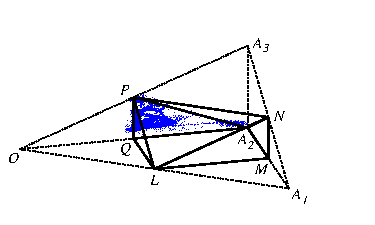
\includegraphics{JCQ-2pulses-polyhedron}
  \caption{Optimized gates in the Weyl chamber. Control with 2 pulses $E_J(t)$
  and $E_{JJ}(t)$. Each blue dot corresponds to one reached gate at final time.
  A 2D subset of the Weyl chamber can be reached.
  }
  \label{fig:JCQ-2pulses_weyl_paths}
\end{figure}
%
In order to also allow the implementation of gates in other parts of the Weyl
chamber we relax the constraint
$E_{JJ}(t)=E_J(t)$ and control both pulses independently.
Figure~\ref{fig:JCQ-fidelity-2pulses} shows the optimization success of the
perfect-entanglers functional for different gate durations in terms of
Eq.~(\ref{eq:FUtilde-lec}), for optimization towards a given local equivalence
class, and Eq.~(\ref{eq:FUtilde-pE}), for optimization towards the polyhedron of
perfect entanglers. The figure shows the resulting fidelity error
$\errPE(\tilde U)=1-F_{\PE}(\tilde{U})$ for optimization towards the polyhedron of
perfect entanglers (blue, squares) and compares it to the fidelity error
$\errLec(\tilde U)=1-F_{\lec}(\tilde{U})$ for optimization towards a specific perfect
entangler equivalence class. Again the operation errors are plotted as
a function of the gate time scaled by the charge energy $E_C T$, that works
against leakage to higher levels.
This time we examined four corners of the polyhedron, namely $Q$ (red, circles),
$A_2$ (yellow, triangles pointing upwards), $P$ (black, triangles pointing
downwards), and also $N$ (gray, diamonds). Clearly the best results again are
the ones for perfect entangler optimization. This time apart from $Q$ and $A_2$
also $P$ can be reached with pretty high fidelity, but $N$ (not shown in
Fig.~\ref{fig:JCQ-fidelity-1pulse}) still can not be reached at all. This is
also supported by Fig.~\ref{fig:JCQ-2pulses_weyl_paths} that shows the position in
the Weyl chamber of the gates reached during optimization. Each blue dot
corresponds to one reached gate at final time. This time a 2D subset of the Weyl
chamber (one border wall of the polyhedron of perfect entanglers) can be
reached.


\subsection{Optimization of Transmon Qubits}
\label{subsec:SC}

For the system of two transmons described in Sec.~\ref{subsec:pe_transmon_model},
we analyze the performance of the perfect entanglers functional using Krotov's
method, as described in Sec.~\ref{sec:Krotov}. The optimization is done for
different gate durations between 25 and 400~ns, starting from a $\sin$-squared
pulse of 35~MHz peak amplitude.

\begin{figure}[tb]
  \centering
  \includegraphics{weyl_paths}
  \caption{Optimized gates in the Weyl chamber, for two transmon qubits,
  optimized with Krotov's method for the perfect-entangler (PE) functional in
  Eq.~(\ref{eq:J_pe_tilde}). The point at which each optimization enters the PE
  polyhedron, or the end point of the optimization of not PE can be achieved,
  is shown in red and labeled with the gate duration.
  The entire optimization path for  $T=400$~ns and $T=50$~ns is shown in blue
  and purple, respectively, with the starting points labeled as 400$^*$ and
  50$^*$.
  The polyhedron of perfect entanglers  is shown in gray. Both the points $O$
  and $A_1$ are coordinates of the identity and are the outer point of the $W_0$
  and $W_0^*$ region of the Weyl chamber region, respective; $A_3$ is the
  coordinate of the SWAP gate and the outer point of the $W_1$ region.
  }
  \label{fig:transmon_weyl_paths}
\end{figure}
%
Fig.~\ref{fig:transmon_weyl_paths} shows the result of the optimization in the
Weyl chamber. The point at which each optimization enters the perfect-entanglers
polyhedron, is indicated in red and labeled
with the gate duration. For $T<50$~ns, no perfect entangler can be reached, and
the end points of the optimization are shown. In
addition, the optimization path for $T=50$~ns, i.e.\ the gate at the quantum
speed limit, and the path for best obtained gate for the longest duration of
$T=400$~ns are traced in blue and purple, respectively. The starting points of
these baths are labeled with the gate duration and an asterisk. Both
optimizations start
in the $W_0^*$ region (near the $A_1$ point). However, the guess pulse for
$T=50$~ns is significantly farther away from the surface of the
perfect-entanglers-polyhedron than the guess pulse for $T=400$~ns (as measured
by $F_{\PE}$, which is maximal at $A_1$ and decreases both in the direction of
the $c_1$-$c_2$ bisector and the $c_3$ axis). Consequently, the optimization for
$T=400$~ns moves directly towards the $W_0^*$ face of the
perfect-entanglers-polyhedron, whereas the optimization for $T=50$~ns enters the
ground surface and emerges the $W_0$ region, before finally
reaching the $W_0$ face of the perfect entanglers. The same general behavior
holds for the other gate durations not shown here: For durations $< 100$~ns,
the optimization enters into $W_0$ from $W_0^*$, whereas longer gate duration
stay within $W_0^*$ entirely.  Thus, different starting points yield different
perfect entanglers.

It is important to realize that the Weyl paths shown in
Fig.~\ref{fig:transmon_weyl_paths} are for the unitarization of the evolution
induced by the pulse in the logical subspace. The starting points of each
optimization will generally include loss from the logical subspace and therefore
cannot be placed uniquely in the Weyl chamber. This accounts for the non-direct
path of the optimization, especially for short gate durations.

\begin{figure}[tb]
  \centering
  \includegraphics{tm_conv_LI}
  \caption{Comparison of optimization success using the perfect entangler (PE)
  functional, Eq.~(\ref{eq:J_pe_tilde}) and the local-invariants functional,
  Eq.~(\ref{eq:J_LI_tilde}), for several points in the Weyl chamber. The label
  A refers to the point $A_2$. The optimization success is evaluated according
  to $\errLec(\tilde U) = 1-F_{\lec}(\tilde U)$ for the local invariants
  optimization and $\errPE(\tilde U) = 1-F_{\PE}(\tilde U)$ for the PE
  optimization, cf.\ Eqs.~(\ref{eq:FUtilde-lec},~\ref{eq:FUtilde-pE}), and is
  shown after a fixed number of iterations using Krotov's method. The
  dark-colored lines, referenced in the legend, show the optimization success
  after 500 iterations, with weight $w=0.1$ for the main part of the functional.
  The lighter lines of same line style and same marker style but larger
  marker size show the optimization success after another 500 iterations, with
  $w=0.01$. Note that for longer gate durations, the optimizations with the
  local-invariants functional are largely converged, such that the lines for 500
  and 1000 iterations are nearly superimposed.
  }
  \label{fig:tm_conv_LI}
\end{figure}
It is instructive to compare the optimization success of the perfect entangler
functional, Eq.~(\ref{eq:J_pe_tilde}) with the optimization under the
local-invariants functional, Eq.~(\ref{eq:J_LI_tilde}) for a few select points
of the Weyl chamber, as was done in Sec.~\ref{subsec:JCQ}. This is shown in
Fig.~\ref{fig:tm_conv_LI}. For comparability with the results of
Sec.~\ref{subsec:JCQ}, the optimization success is shown as $1-F_{\lec}$ for the
local invariants optimization, and $1-F_{\PE}$ for the perfect-entanglers
optimization, see. Eqs.~(\ref{eq:FUtilde-lec},~\ref{eq:FUtilde-pE}). That is,
quantities used in the plot to evaluate the optimization success (in $c$-space)
differ from the functional that was used in the optimization (in $g$-space). The
shown $c$-space quantities also have the benefit of being in the range $[0,1]$,
and thus can nicely be interpreted as a fidelity/error measure. The optimization
success is shown after a fixed number of 500 iteration. In order to indicate to
which degree these results are converged, the results after another 500
iteration, with increased weight on the unitarity term of the functional, is
shown in lighter color for each curve.

The results of Fig.~\ref{fig:tm_conv_LI} show how different gates are easiest to
reach for different gate durations. In agreement with the results of
Fig.~\ref{fig:transmon_weyl_paths}, for durations $< 50$~ns, a speed limit
(i.e.\ jump in the optimization error) can be seen. For short gate durations,
optimization towards the point $Q$ in the Weyl chamber is most successful. This
matches the optimized gates for $T \le 100$~ns in
Fig.~\ref{fig:transmon_weyl_paths} being near the $Q$ point. Also correspondingly,
the longer gate durations end near the $N$ point. The failure to reach the point
$Q$ in the Weyl chamber is due to the symmetry-structure of the Weyl chamber.
Namely, for the ground surface of the chamber, there is a mirror axis defined
by the line through $L$ and $A_2$, where mirrored points are in the same local
equivalence class. Both the $Q$-point and the $M$ point have local invariants of
$g_1 = \frac{1}{4}, g_2=0, g_3=1$. Since the optimization was performed in
$g$-space, these two points are not distinguishable; indeed, for long gate
durations, the $Q$-optimization successfully reached the $M$ point. For the
local-invariants optimization, reaching the $A_2$ point is in some sense hardest,
since it on the opposite end of the perfect entanglers polyhedron, starting from
$O$ or $A_1$. This is reflected in the still significant improvement between
iterations 500 and 1000 in the green short-dashed curve, whereas the other
optimizations are effectively converged after 500 iterations.
In comparison with the local-invariants optimization, using the perfect
entanglers functional shows excellent performance. It automatically identifies
the optimal gate for a given gate duration and reaches significantly better
fidelities. This is due to the fact that a perfect entangler can usually be
reached in just a few tens of iterations, and the remainder of the optimization
then focuses on improving the unitarity of the obtained gate. Also, unlike the
local-invariants optimization, it does not show any slow-down in the convergence
rate. While in principle (due to the full controllability of the system), the
direct optimizations should also yield arbitrarily small gate errors, as long as
the gate duration is above the quantum speed limit, in practice this depends
heavily on numerical parameters such as the weight $\lambda_a$ in Krotov's
method and would take an infinite number of iterations. The perfect-entangler
optimization shows remarkable robustness with respect to this issue.

\begin{figure}[tb]
  \centering
  \includegraphics{tm_conv_favg}
  \caption{Success of optimization of 2 transmon qubits using Krotov's method.
  The population from the logical subspace is shown in light red, the
  concurrence of the closest unitary gate $\Op{U}$ induced in the logical
  subspace in blue, and the gate fidelity with which $\Op{U}$ is implemented in
  light red.}
  \label{fig:tm_conv_favg}
\end{figure}
The values of the optimization error in Fig.~\ref{fig:tm_conv_LI} of $10^{-3}$
or $10^{-2}$ should not be understood to indicate a gate error of that
magnitude, which would be well above the quantum error correction threshold.

Fig.~\ref{fig:tm_conv_favg} shows the optimization success of the
perfect-entanglers functional for different gate durations in terms of more
physical quantities, i.e.\ the
generated entanglement and the average gate fidelity. The ``target'' gate with
respect to which the gate fidelity is calculated is the closest unitary gate $U$
to the non-unitary $\tilde U$ projected from the full Hilbert space. For $T
> 50$~ns, the gate errors are at or below $10^{-4}$. We may also get some
insight into the breakdown of the optimization once the quantum speed limit is
reached. The blue dashed curve shows the concurrence error $1-C$ of the gate
$U$. For short gate durations, insufficient entanglement is generated, while for
$T > 50$~ns, the gate is a perfect entangler, with a concurrence of exactly 1.
The only source of gate error is then the loss of population from the
logical subspace, shown in light red in Fig.~\ref{fig:tm_conv_favg}.
The average gate fidelity with which $\Op{U}$  is realized is completely
determined by the non-unitarity, as can be
seen from the two curves being completely
superimposed. For longer gate durations, the optimization yields exponentially
more unitary gates.
